\section{FreeRTOS}
\begin{figure}[H]
    \centering
    
\includegraphics[width=0.3\textwidth]{figures/FreeRTOS.png}
    \caption[Ícono de FreeRTOS]%
            {Ícono de FreeRTOS \citep{img_FreeRTOS}}
    \label{fig:sistema_operativo_FreeRTOS}
\end{figure}
FreeRTOS es un sistema operativo en tiempo real con un kernel planificador, desarrollado para ejecutarse con microcontroladores. Está compuesto funcionalidades de planificación en tiempo real, comunicación entre tareas, análisis temporal y primitivas de sincronización con el propósito de cumplir con las tareas con el plazos estrictos de ejecución \citep{He2020}.
En cuanto a su arquitectura hace uso de un microkernel para administrar tareas en tiempo real, casi similar al RTLinux en que admiten núcleo dual, lo que permita separar tareas critica y no criticas \citep{Serino2019} Esta escrito en lenguaje C estándar y con algunas lineas de código en ensamblador para que se acople a diferentes arquitecturas.
Dentro de su componentes claves tenemos el \textbf{planificador}, \textbf{mecanismos de comunicación}, \textbf{sincronización} gracias al uso de colas y semáforos. Incluyendo la estructura de \textbf{Task Control Block (TCB)} para la administración de procesos y tareas \citep{Barry2018}.
\begin{figure}[H]
    \centering
    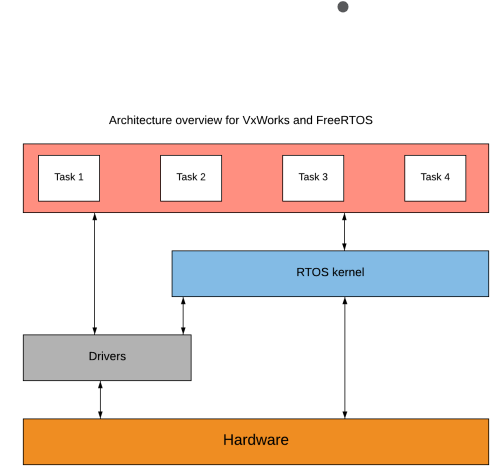
\includegraphics[width=0.3\textwidth]{figures/ArquitecturaFreeRTOS.png}
    \caption[Arquitectura de FreeRTOS]%
            {Diseño de la arquitectura de FreeRTOS \citep{img_FreeRTOS}}
    \label{fig:Disenio_operativo_FreeRTOS}
\end{figure}
FreeRTOS es código abierto con una licencia GPL, lo que permite su uso en aplicaciones comerciales. El código está disponible públicamente y cuenta con documentación extensa en el código fuente en su sitio oficial \citep{FreeRTOS_org}.